\chapter{Food 2}

\begin{itemize}
\tightlist
\item
  \textbf{NP 23,} Over-kept tonics
\item
  \textbf{Pc 31,} Public alms centre
\item
  \textbf{Pc 32,} Four bhikkhus specifically invited
\item
  \textbf{Pc 33,} Meal before invitation
\item
  \textbf{Pc 34,} More than three bowlfuls
\item
  \textbf{Pc 35,} More food after turning down what was offered
\item
  \textbf{Pc 36,} Tricking to break Pc 35
\item
  \textbf{Pc 41,} Handing food to members of other religions
\item
  \textbf{Pc 47,} Exceeding an invitation
\end{itemize}

\section{NP 23, Over-kept tonics}

\includemap{../../src/includes/mindmaps/np-23-tonics.png}

\begin{multicols}{2}

\textbf{Object:} any of the five tonics.

``There are these five tonics -- ghee, butter, oil, honey, and syrup --
that are generally regarded as tonics, serve the purpose of nourishment,
but are not considered as substantial food.''
(\href{https://suttacentral.net/pli-tv-kd6/en/brahmali}{Kd 6})

\textbf{Effort:} one keeps the tonic past the 7th dawnrise after
receiving it.

\textbf{Perception} is not a factor.

If one thinks the 7th dawn haven't passed, but it has, it is still NP.

If one thinks ``I receive \emph{this} salt as food for the morning, and
\emph{this} salt as medicine for later'', it may be a personal practice,
but not part of the rule. It doesn't affect the period of how long the
item may be used by oneself or any other bhikkhu.

\end{multicols}

\clearpage

\textbf{Origin:} Ven. Pilindavaccha receives an abundance of tonics, and
shares with his monks. They begin to ``fill up basins and waterpots and
setting these aside, they filled their water filters and bags and hung
these in the windows. The tonics were dripping all over and the
dwellings became infested with rats.''
(\href{https://suttacentral.net/pli-tv-bu-vb-np23/en/brahmali}{NP 23})

\textbf{Mixing:} The mixture takes on the shortest lifetime of the
ingredients. (Mv. VI.40.3.)

\begin{center}
\begin{tabular}{llllllll}
a. & 1d juice & rec. that morning & + & food & rec. that morning & \(\rightarrow\) & that morning\\
\hline
b. & 7d tonic & rec. that morning & + & food & rec. that morning & \(\rightarrow\) & that morning\\
\hline
c. & lifetime medicine & rec. that morning & + & food & rec. that morning & \(\rightarrow\) & that morning\\
\hline
d. & 7d tonic & rec. sometime & + & juice & rec. that day & \(\rightarrow\) & until dawn\\
\hline
e. & lifetime medicine & rec. sometime & + & juice & rec. that day & \(\rightarrow\) & until dawn\\
\hline
f. & lifetime medicine & rec. sometime & + & 7d tonic & rec. sometime & \(\rightarrow\) & 7 days\\
\end{tabular}
\end{center}

\subsection{7 days}

\emph{Sattāha paramaṃ}, ``up to seven days''. The Vinaya counts days
from dawn to dawn, hence one may use a 7 day tonic \emph{until the 7th
dawn}.

Confusion arises from ``7 days'' meaning either ``for 7 days''
(interval) or ``on the 7th day'' (ordinal).

\vspace*{\baselineskip}
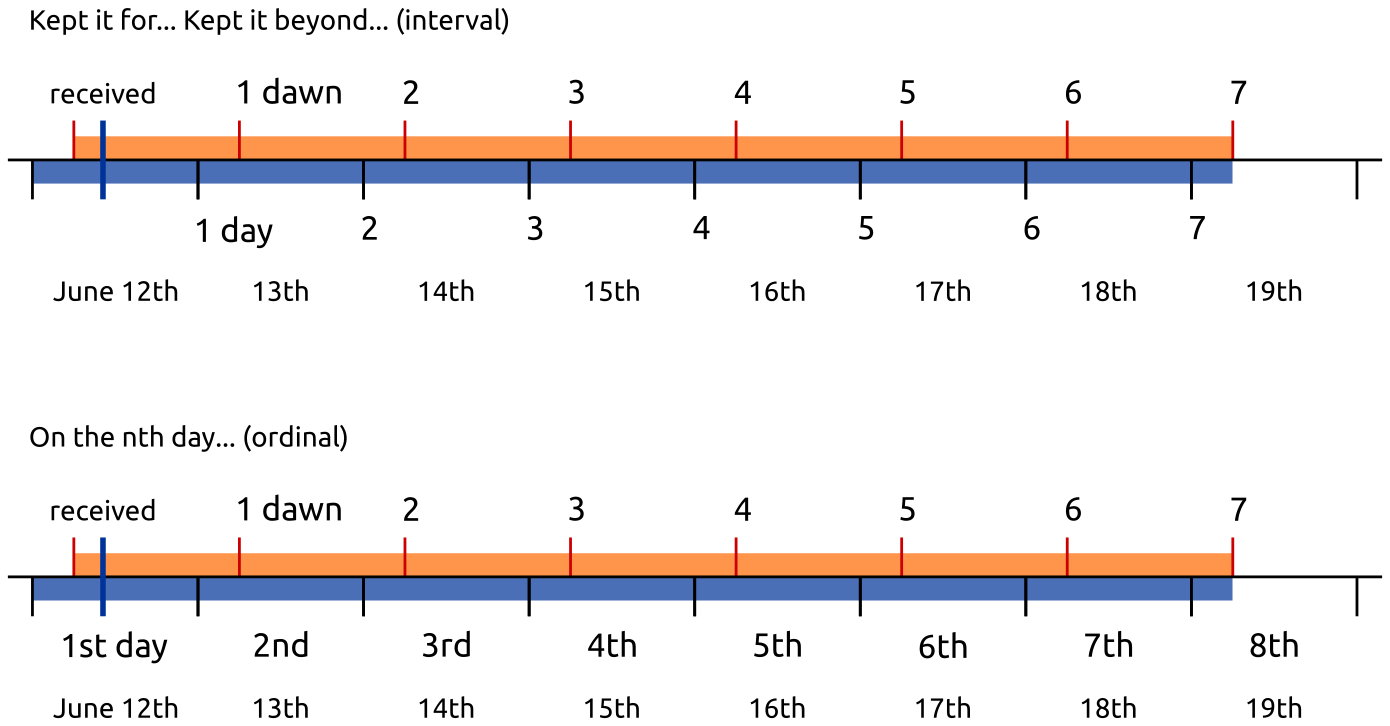
\includegraphics[width=\linewidth]{../../src/includes/figures/7-days.png}

\subsection{Breakfast tray}

After dawn, one receives a tray with bread, jams, honey, butter and
salt. At this point the lifetimes are:

\begin{itemize}
\tightlist
\item
  bread, jams: morning
\item
  honey, butter: 7 days
\item
  salt: lifetime
\end{itemize}

If the knife which one used carries bread morsels or jam into the honey
or the butter, these will be only allowable in the morning.

If one is careful to clean the knife and avoid mixing, one may use them
on the bread and keep the rest until their allowed lifetimes.

The next day, one receives a tray with only bread. One may \textbf{not}
mix the allowables from the previous day with the food received today.

Putting the salt, honey or butter (rec. yesterday) on the bread would be
Pc 38 (eating stored food).

\section{Pc 31, Public alms centre}

One may eat one meal at a public alms centre, not two or more days in a
row.

Origin: the group of six feel tired of almsround and keep going to the
same public kitchen.

Soup kitchens, homeless shelters, etc. Any place where all comers are
offered food free of charge.

\subsection{Non-offences}

\begin{itemize}
\tightlist
\item
  one is invited by the owners
\item
  being ill (not being able to leave)
\item
  the food is intended for bhikkhus
\item
  the centre limits the amount of food one may take (thus being able to
  censure a greedy person)
\end{itemize}

\section{Pc 32, Four bhikkhus specifically invited}

Origin: Devadatta was telling householders which bhikkhu to give alms
to, in order to form his own faction within the Sangha.

A `group meal' here means four or more bhikkhus, specifically named in
the invitation, out of the entire community.

There is no offence if the invitation is for `x number of bhikkhus',
leaving the selection to the community.

\section{Pc 33, Meal before invitation}

Origin: some bhikkhus are concerned about the food at a meal invitation,
and go alms-round nonetheless. There is plenty of food at the
invitation, but they can't eat any more.

See
\href{https://www.accesstoinsight.org/tipitaka/kn/snp/snp.4.16.than.html}{Snp
4.16}, on how to train oneself: ``He should conquer these four thoughts
of lament: `What will I eat, or where will I eat. How badly I slept.
Tonight where will I sleep?'\,''

No offence is the donors are informed, e.g.~that the bhikkhus will eat
breakfast before the midday meal. It is nonetheless bad manners to eat
so much at breakfast to not be able to eat at the meal.

If the donors are not informed, very light food is still allowed, such
as drinking thin rice porridge.

\section{Pc 34, More than three bowlfuls}

Origin: some bhikkhus don't know moderation in accepting cakes as
provisions from faithful supporters.

After accepting the provisions, the bhikkhu should inform the other to
not accept more at that place. It is a \emph{dukkaṭa} offence to not do
so.

The term `provisions' here refers to food prepared for \emph{someone
else} going on a journey. Hence there is no offence if the food was
prepared \emph{for the bhikkhu}, although restraint should be exercised.

\section{Pc 35, More food after turning down what was offered}

Origin: some bhikkhus selectively accept some alms-food from one donor,
then go to another donor to have something else they like. The first
donor could have offered all the food they needed, and feels hurt that
they went somewhere else for more.

If the bhikkhus already accepted all that the donor wanted to give, it
is not an offence to seek more alms if they would need more food.

The donor may offer more food, and they may accept or refuse certain
items while still eating.

If they have finished eating, and they had refused more food while
eating, they can't accept more food items which are not leftovers.

If they have finished eating, but they \textbf{had not} refused more
food while eating, they may accept more food items.

\subsection{Non-offences}

\begin{itemize}
\tightlist
\item
  accepting for the sake of another
\item
  accepting the leftovers of another
\end{itemize}

\section{Pc 36, Tricking to break Pc 35}

Origin: one bhikkhu, having been criticized for his bad behaviour,
contrives a situation for the other bhikkhu to break Pc 35.

\textbf{Intention} has to be wishing to find fault and blame the other
bhikkhu.

No offence for giving him leftover food to eat.

\section{Pc 41, Handing food to members of other religions}

One places oneself in the position of the followers of other religions.

It is not an offense to prepare food in a tray and placing it so that
they can help themselves.

\section{Pc 47, Exceeding an invitation}

When an invitation is made that one may ask for certain requisites, one
may use it until four months, unless it has been repeated, or is a
permanent invitation.

\subsection{Non-offenses}

\begin{multicols}{2}

\begin{itemize}
\tightlist
\item
  from relatives
\item
  for the sake of another
\item
  from one's own resources
\item
  being ill, if one shows consideration
\end{itemize}

\end{multicols}

``The time period for which we were invited has passed, but we have need
of medicine.''

